\documentclass[times, utf8, seminar]{fer}
\usepackage{booktabs}

\setlist[description]{leftmargin=\parindent,labelindent=\parindent}

\begin{document}

% TODO: Navedite naslov rada.
\title{Faza konsenzusa u OLC paradigmi sastavljanja genoma}

% TODO: Navedite vaše ime i prezime.
\author{Ivan Paljak, Ivan Sekulić}

% TODO: Navedite ime i prezime mentora.
\voditelj{Mile Šikić}

\maketitle

\tableofcontents

\chapter{Uvod}

Proučavanje strukture DNA u fokusu je znanstvenika od samog otrkića DNA.
Precizno čitanje genoma predstavlja velik izazov te su s vremenom razvijani sve brži i jeftiniji uređaji za što bolja očitanja.
Danas su uređaji i dovoljno brzi i jeftini, ali se javlja problem kratkih očitanja.
Bioinformatika, između ostalog, teži spojiti ta kratka očitanja u jedinstvenu sekvencu (genom).

Prilikom sastavljanja genoma, javlja se nekoliko problema.
Prvi je nepreciznost uređaja za sekvenciranje, što zahtjeva višestruka očitanja jednog genoma kako bi se, određenim metodama, mogao ustanoviti stvarni niz.
Također, danas se koriste metode temeljene na \emph{shotgun} sekvenciranju cijelog genoma pri čemu nemamo nikakvu informaciju o poretku pojedinih očitanja.
Treći otežavajući faktor uspješnog sastavljanja jedinstvene sekvence jest varijabilna duljina očitanja.
Uređaji druge generacije, koji treutno prevladavaju, rade očitanja veličine od nekoliko desetaka do par stotina nukleotida.
Treća generacija uređaja proizvodi dulja očitanja, od nekoliko tisuća nukleotida, ali imaju velik postotak pogreške -- od 15\% do čak 40\%.

Razvijeno je nekoliko algoritama koji se bave problemom sastavljanja genoma, a najkorišteniji su oni temeljeni na algoritmima nad grafovima.
Najčešće se koristi jedna od dviju osnovnih metoda: Preklapanje-Razmještaj-Konsenzus \emph{engl. Overlap-Layout-Consensus, OLC} metode temeljene na grafu preklapanja ili metode temeljene na \emph{de Bruijn} grafovima \citep{sikic2013bioinformatika}.
U ovom projektu, bavimo se konsenzus fazom OLC paradigme.

Ovaj dokument organiziran je na sljedeći način: u sljedećem poglavlju opisan je algoritam koji smo koristili za dobivanje konsenzusa.
Poglavlje \ref{sec:implementacija} kratko opisuje našu konkretnu implementaciju i karakteristike korištenih računala.
U poglavlju \ref{sec:eval} dana je usporedba vlastite implementacije s referentnim radom.
Poslijednje poglavlje sadrži zaključak cjelokupnog projekta.




\chapter{Algoritam Sparc}

Cilj ovog projekta bio je implementirati algoritam Sparc \citep{ye2016sparc} koji se koristi u konsenzus fazi preklapanje-razmještanje-konsenzus (engl. Overlap-Layout-Consensus, OLC) pristupa.
Kod OLC pristupa, traženje puta u grafu svodi se na traženje Hamiltonovog puta.
To je put koji prolazi kroz sve vrhove u grafu točno jedanput te bi nam takav put otkrio cijeli slijed.
Traženje Hamiltonovog puta je NP potpun problem te je potrebno uvesti heuristike za pojednostavljenja grafa.
Sparc je algoritam za konsenzus fazu OLC pristupa, temeljen na \emph{k-mer/de Bruijn} \citep{hannenhalli1996positional} grafovima.

\section{Ulaz u algoritam}
Algoritam koristi izlaz iz faze razmještanja OLC pristupa te sva početna očitanja genoma.
Očitanja su mapirana na kontigu iz faze razmještanja i pohranjena u datoteku formata .sam, opisanom u nastavku.

Kako bi uspješno izgradili graf i proveli algoritam, potrebno je znati gdje se pojedina očitanja mapiraju na osnovnu kontigu.
Te informacije dobivano iz .sam datoteke koju smo generirali alatom \emph{GraphMap} \citep{sovic2016fast}.
Nama najvažnije informacije u datoteci jesu:
\begin{itemize}
  \item POS: pozicija na osnovnoj kontizi na kojoj počinje mapiranje pojedinog očitanja
  \item CIGAR: operacije obavljene nad očitanjem kako bi se dobilo mapiranje (dodavanje, brisanje, pomicanje, itd.)
  \item SEQ: očitana sekvenca u prvotnom obliku (bez obavljenih CIGAR operacija)
  \item QUAL: kvaliteta očitanja (iz .fastq datoteke očitanja)
\end{itemize}

Važnost navedenih informacija bit će jasnija kasnije.
Za naše potrebe, spremili smo sve važne informacije u zasebnu datoteku koja se sastoji od osnovne kontige (engl. backbone, layout) u prvoj liniji.
U nastavku datoteke su očitanja zapisana kroz tri linije.
Prva linija predstavlja originalno očitanje na koje su primjenjene CIGAR operacije kako bi se dobilo poravnanje s backbone-om.
U drugoj liniji nalazi se kvaliteta očitanja (QUAL), a u trećoj je pozicija na backbone-u na kojoj počinje mapiranje izmjenjene sekvence.

\section{Opis algoritma}
Najprije se gradi graf direktno iz backbone-a, kako je prikazano na slici \ref{fig:sparc.png}.
Linearno se prolazi kroz backbone te se u čvorove stavljaju \emph{k-torke (k-meri)}, a bridovi su definirani kao postojeći, ako su sufiks jednog čvora, a prefiks drugoga. 
Zatim se prolazi kroz mapirana očitanja te se ažuriraju težine u grafu gdje dolazi do preklapanja.
Dodaju se novi čvorovi i bridovi ako se u očitanju javljaju nove k-torke.
Konačni korak je pronalazak najtežeg puta u grafu.
Primjer izgradnje grafa dan je na slici \ref{fig:sparc}.
TODO: objasni bolje

\begin{figure}[htb]
\centering
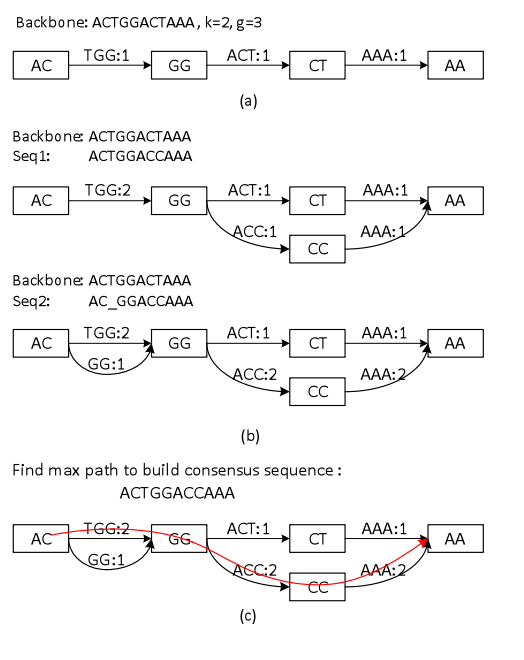
\includegraphics[scale=0.6]{figures/sparc.png}
\caption{Izgradnja grafa.}
\label{fig:sparc}
\end{figure}



\chapter{Implementacija}
\label{sec:implementacija}

\section{Organizacija koda}
Cjelokupni algoritam implementiran je u programskom jeziku C++11.
Implementacija je podijeljena u dva osnovna dijela.
Prvi modul \emph{reading.cpp} učitava sve potrebne podatke (backbone i očitanja u .sam formatu) te primjenjuje CIGAR operacije na pojedina očitanja.
Time generiramo datoteku vlastitog formata.
U prvoj liniji zapisan je backbone, a svake sljedeće tri linije predstavljaju jedno očitanje na način:
\begin{enumerate}
  \item očitanje na koje su primijenjene CIGAR operacije,
  \item kvaliteta očitanja na koju su primijenjene CIGAR operacije,
  \item pozicija u backbone-u na koju se mapira očitanje.
\end{enumerate}

Drugi modul \emph{sparc.cpp} direktna je implementacija algoritma Sparc prema ideji objašnjenoj u odgovarajućem poglavlju. 

\section{Kofiguracija korištenog računala}

Računalo korišteno pri pokretanju cjelokupnog pipelinea ima sljedeću konfiguraciju:
\begin{description}
  \item [OS] Linux 14.04.1-Ubuntu x86\_64
  \item [Procesor] Intel(R) Core(TM) i7-5820K CPU @ 3.30GHz (CPUs: 12)
  \item [RAM] 32Gib @ 2133 MHz
\end{description}



\chapter{Evaluacija}

\secton{DnaDiff iz Mummer paketa}

ne radi

\section{Usporedba vlastitog rješenja s referentnim radom}

Lošije je.



\chapter{Zaključak}

U okviru ovoga projekta upoznali smo se s osnovama bioinformatike.
Proučili smo OLC paradigmu sastavljanja genoma te implementirali algoritam temeljen nad grafovima za konsenzus fazu paradigme.
Uočili smo određene probleme sastavljanja genoma te se upoznali s postupcima i najčešće korištenim alatima u bioinformatici.

Impementiran je algoritam \emph{Sparc} te je napravljena analiza rezultata.
Postignuto je značajno poboljšanje u odnosu na početnu sekvencu, ali nisu dostignuti rezultati originalnog algoritma.
Kompletan kod, upute za instalaciju i pokretanje mogu se pronaći na github.com/ipaljak/bioinfo.




\bibliography{literatura}
\bibliographystyle{fer}

\chapter{Sažetak}
Ovaj projekt napravljen je za kolegij Bioinformatika na FER-u.
Implementiran je algoritam \emph{Sparc} za generiranje konsenzusa u OLC paradigmi sastavljanja genoma.
Dobiveni su rezultati te uspoređeni s referentnim radom.

\end{document}
